\section{算子与内核：GEMM、FlashAttention 与融合}
\label{sec:kernel}

Transformer 的 FLOPs 绝大部分在 GEMM 里，而端到端时间的相当一部分却花在访存受限的「小算子」和 attention 的中间矩阵上。
本节先推导 GEMM 分块的复用与上界，再详细讨论 FlashAttention 三个版本以及一个经常被误解的问题——
它到底把 HBM 流量降了多少，最后讨论融合与 Triton。

\subsection{GEMM 的算术强度与分块}

$C_{M\times N}=A_{M\times K}B_{K\times N}$ 的运算量为 $F=2MNK$（一次乘加记 2 FLOP，厂商峰值也按此计）。若三个矩阵各过一次 HBM，
\begin{equation}
\begin{gathered}
I_{\text{GEMM}} = \frac{2MNK}{s(MK+KN+MN)},\\
I_{\text{square}} = \frac{2n}{3s},\qquad
I_{\text{GEMV}} \approx \frac{2}{s},
\end{gathered}
\end{equation}
其中 $s$ 为每元素字节数。BF16 方阵的强度为 $n/3$，在 H100 上要 $n\gtrsim 900$ 才越过拐点 295；
GEMV（$M=1$）只有 1~FLOP/B，只能用到峰值的 1/295。这一个式子解释了 decode 为什么慢、为什么 batch 是推理吞吐的第一杠杆。

上式假设「每个矩阵只过一次 HBM」，这要求片上能放下足够大的块。设快存可放 $M_s$ 个元素，采用 $b\times b$ 方块且三块同时驻留，
则 $3b^2\le M_s$。每加载两个 $b\times b$ 块做 $2b^3$ 次运算，局部强度约为 $b/s$；总访存
\begin{equation}
Q \approx \frac{2n^3}{b}+n^2 = \Theta\!\left(\frac{n^3}{\sqrt{M_s}}\right),
\end{equation}
与 Hong--Kung 下界同阶~\cite{hong1981io}。

\begin{est}{H100 一个 SM 的 shared memory 能支撑多大的 GEMM 块？}
H100 每 SM 最多 228~KB shared memory。BF16 下 $3b^2\times2\le228$~KB 得 $b\le197$，工程上取 128。此时单个 block 的局部强度
$b/s=64$~FLOP/B，\emph{还不到}拐点 295。真实 kernel 靠三件事越过拐点：多个 thread block 在 50~MB 的 L2 中共享 A、B 的同一行块/列块
（L2 带宽约为 HBM 的 3 倍）；非方形块（如 $128\times256$）；以及寄存器层再分块。这说明面试中「块越大越好」的回答不完整：
块大小受 shared memory、寄存器、occupancy 与 SM 数量（块数要足以填满 132 个 SM）的共同约束。
\end{est}

\lab{CS149 A4}在一个带 SBUF/PSUM 容量约束的 Trainium 式分块模型上验证了同样的规律：$4096^3$ 的 BF16 GEMM，
tile 边长从 128 增至 256、512 时 HBM 强度为 63.0、124.1、240.9~FLOP/B，约等于边长的一半；SBUF $\ge$1~MiB 之后，
2~MiB 的 PSUM（FP32 累加器）把强度封顶在 315.1；再增大 SBUF 只能加大 $t_k$、把 DMA 次数从 2080 降到 96，不再提高强度。
这些加速器参数是模型假设，不能当成 Trainium 规格（第~\ref{sec:accel} 节）。

\begin{qa}{矩阵乘分块时块大小怎么选？}
\ans 四个约束：（1）容量：$3b^2 s\le M_s$（双缓冲时再减半）；（2）强度：局部强度约 $b/s$，需结合 L2 复用越过拐点；
（3）并行度：$(M/b_m)(N/b_n)$ 个块要足以填满所有 SM，小矩阵常用 split-K；（4）硬件形状：块要是 MMA 指令形状的整数倍，
并兼顾 occupancy 与寄存器压力。最终由 autotuning 在候选集合中选。
\wrong 「越大越好」；或只考虑 shared memory 容量而忽略 SM 数与波次（wave quantization）。
\end{qa}

\textbf{MFU}（model FLOPs utilization）是训练效率的标准口径~\cite{chowdhery2022palm}：
$\mathrm{MFU}=6N\cdot(\text{tokens/s})/(n_{\text{GPU}}P_{\text{peak}})$。例如 8 张 H100 训练 7B 模型达到每秒 $10^5$ token，
MFU $=6\times7\times10^9\times10^5/(8\times989\times10^{12})\approx 53\%$。HFU 把重计算的 FLOPs 也算进去，所以 $\mathrm{HFU}\ge\mathrm{MFU}$。
MegaScale 报告在 12,288 张 GPU 上训练 175B 模型达到 55.2\% MFU~\cite{jiang2024megascale}，可作为大规模训练 MFU 的参考量级。

\begin{qa}{batch=1 的矩阵--向量乘为什么在任何 GPU 上都慢？}
\ans BF16 GEMV 的强度约为 1~FLOP/B，H100 拐点 295，只能用到峰值的 0.3\%。提高强度只有两条路：增加 batch（GEMV 变 GEMM），
或减少每个权重的字节数（量化）。换更快的卡帮助有限：H100 相对 A100 带宽只多 1.6 倍。
\wrong 「decode 慢是因为计算量大」。
\end{qa}

\subsection{Attention 的代价}

单头 attention 中 $Q,K,V\in\mathbb{R}^{T\times d}$，$S=QK^\top$ 与 $O=PV$ 各需 $2T^2d$ FLOPs，多头合计每层前向
$4T^2d_{\text{model}}$；朴素实现要物化 $T\times T$ 的 $S$ 与 $P$，每层每样本显存 $h\,T^2 s$ 字节。

\begin{est}{8K 上下文的 attention 占多少计算和显存？}
$T=8192$、$d_{\text{model}}=4096$、32 头、BF16：attention 前向 $4T^2d_{\text{model}}=4\times8192^2\times4096\approx1.1$~TFLOP/层；
同层投影与 MLP 约 $24Td_{\text{model}}^2\approx3.3$~TFLOP（按 4 倍 MLP 估），attention 约占 1/4。分数矩阵 $32\times8192^2\times2$~B
$\approx4.3$~GB/层/样本，反传还要保存。结论：中等长度下 attention 的问题首先是\emph{显存与 IO}，其次才是 FLOPs；
这正是 FlashAttention 的出发点。
\end{est}

\subsection{Online softmax 与 FlashAttention}

softmax 看似需要整行的最大值与和。Milakov 与 Gimelshein 的 online normalizer~\cite{milakov2018online} 观察到
$e^{x-m_{\text{new}}}=e^{x-m_{\text{old}}}\cdot e^{m_{\text{old}}-m_{\text{new}}}$，于是两段的统计量 $(m_i,\ell_i,o_i)$ 可以合并：
\begin{equation}
\begin{aligned}
m &= \max(m_1,m_2),\quad
\ell = e^{m_1-m}\ell_1 + e^{m_2-m}\ell_2,\\
o &= e^{m_1-m}o_1 + e^{m_2-m}o_2,\qquad O=o/\ell .
\end{aligned}
\label{eq:online}
\end{equation}
Rabe 与 Staats 据此证明 self-attention 只需 $O(\sqrt{n})$ 乃至 $O(\log n)$ 的额外显存~\cite{rabe2021selfattention}；
FlashAttention~\cite{dao2022flashattention} 把它与 GPU 存储层次结合：把 $Q$ 切成 $B_r$ 行一块、$K,V$ 切成 $B_c$ 行一块，
$S$、$P$ 的块只在 SRAM 中存在，反向传播保存每行的 logsumexp $L_i=m_i+\log\ell_i$，按块重算 $P_{ij}=\exp(S_{ij}-L_i)$。
它是\emph{精确}算法，不减少 FLOPs（反向还多一次 $QK^\top$ 重算），省的是 HBM 读写与显存：额外显存从 $O(T^2)$ 降到 $O(T)$。

\textbf{IO 复杂度}。SRAM 可放 $M$ 个元素，要同时放下 $K_j,V_j$ 与 $Q_i,O_i$，论文取 $B_c=\lceil M/4d\rceil$、
$B_r=\min(\lceil M/4d\rceil,d)$。外层每遍历一个 $K/V$ 块就要扫一遍全部 $Q,O$，总访问量
\begin{equation}
Q_{\text{flash}} = \Theta\!\left(\frac{T^2d^2}{M}\right),
\end{equation}
并且论文证明没有精确算法能在全部 $M\in[d,Td]$ 上做到 $o(T^2d^2/M)$~\cite{dao2022flashattention}。
关键在于：$d=64$--128、$M\approx10^5$ 时 $d^2/M$ 是一个常数（约 0.04--0.16），\emph{流量在 $T$ 上仍是二次的}，只是常数比朴素实现小。

\begin{figure*}[!t]
\centering
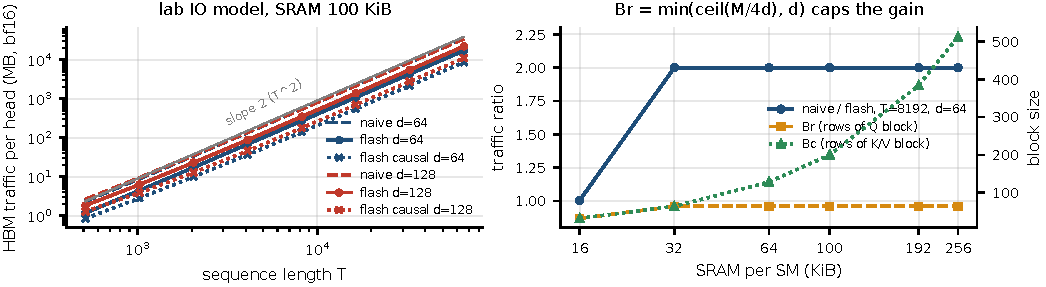
\includegraphics[width=\textwidth]{fig_lab_flash}
\caption{本文配套实验（CS229S P1）的 FlashAttention IO 计数器结果。左：每头 HBM 流量随 $T$ 的变化（BF16，SRAM 100~KiB），
朴素实现只计 $S$、$P$ 各读写一次；所有曲线斜率均为 2，即 $\Theta(T^2)$。非因果时 Flash 只比朴素少 2.00 倍（$d=64$）或 1.56 倍（$d=128$），
因果时由于跳过上三角块约少 4 倍。右：$T=8192,d=64$ 时流量比随 SRAM 的变化。$B_r$ 在 32~KiB 处即被 $d$ 截住，
更大的 SRAM 只增大 $B_c$，不再减少 $K/V$ 的重读次数。IO 计数器与解析模型在 8 组配置上逐元素一致。}
\label{fig:labflash}
\end{figure*}

图~\ref{fig:labflash} 是这一结论的直接证据。配套实验用 numpy 实现了 FA2 顺序的分块前向与基于 logsumexp 的反向，
float64 下 $O$、$dQ$、$dK$、$dV$ 与 \texttt{torch} 自动微分的最大误差 $\le4.9\times10^{-15}$；IO 计数器记录每次块读写。
$d=64$、$T=65536$ 时朴素 34,393~MB、Flash 17,197~MB，比值 2.00；$d=128$ 时 1.56。这与白板公式吻合：
Flash 流量 $\approx 2Td\cdot(T/B_r)+4Td$，朴素 $\approx4T^2$，比值 $\approx 2B_r/d$，$B_r=d$ 时为 2。
\emph{不能}由此推出「FlashAttention 在 GPU 上只快 2 倍」：真实 eager 实现中 scale、mask、softmax、dropout 各自对 $T^2$ 张量读写一次，
$S$ 常以 FP32 存储，且 $K/V$ 的重读在 GPU 上大多命中 L2；FlashAttention 最确定的收益是显存从 $O(T^2)$ 到 $O(T)$
以及消除这些中间 kernel。同样，numpy 版 Flash 比朴素版更慢（$T=1024,d=128$ 时 44.6 对 22.9~ms），这是 Python 循环开销，与 GPU 无关。

\begin{qa}{FlashAttention 快在哪？它减少了 FLOPs 吗？HBM 访问降到线性了吗？}
\ans 没有减少 FLOPs，反向还多一次重算；它是精确算法。快在不把 $T\times T$ 的分数矩阵写回 HBM：分块计算，用 online softmax 维护每行最大值与分母，
把 matmul--softmax--matmul 融合成一个 kernel。显存从 $O(T^2)$ 降到 $O(T)$；HBM 访问是 $\Theta(T^2d^2/M)$，对常见 $d$ 在 $T$ 上仍是二次，
只是常数显著变小。
\wrong 「它是近似 attention」；「访存从二次降到线性」——只有显存是线性的。
\end{qa}

\textbf{FlashAttention-2}~\cite{dao2024flashattention2} 的改动全部是工程性的（表~\ref{tab:fa}）：外层循环改为遍历 $Q$ 块，
每个 thread block 负责一段 $Q$，输出累加器留在寄存器、最后只写一次；推迟 rescale，只存 logsumexp，减少非矩阵乘 FLOPs
（A100 上非 tensor-core FLOP/s 比 tensor core 低约 16 倍）；除 batch 与 head 外还沿序列长度并行，长序列小 batch 时也能填满 SM；
block 内把 $Q$ 切给 4 个 warp，避免 v1 中 warp 间经 shared memory 归约。论文报告在 A100 上达到理论峰值的 50--73\%。

\textbf{FlashAttention-3}~\cite{shah2024flashattention3} 面向 Hopper：producer warp 只发 TMA 加载，consumer warpgroup 做 wgmma 与 softmax
（warp specialization）；两个 consumer warpgroup ping-pong，使一个做 softmax 时另一个做 GEMM；同一 warpgroup 内也让 softmax 与下一块 GEMM 重叠；
FP8 路径用分块量化与 Hadamard 变换（incoherent processing）压低离群值误差。论文报告 H100 上 BF16 约 740~TFLOP/s（约 75\% 利用率）。

\begin{table}[!t]
\centering
\caption{FlashAttention 三个版本的对比}
\label{tab:fa}
\footnotesize
\begin{tabularx}{\columnwidth}{@{}l Y Y Y@{}}
\toprule
 & FA1 (2022) & FA2 (2023) & FA3 (2024) \\
\midrule
目标硬件 & A100 等 & A100 & H100 (Hopper) \\
外层循环 & $K/V$ 块 & $Q$ 块 & $Q$ 块 \\
$O$ 的写回 & 每个 $K/V$ 块读写一次 & 只写一次 & 只写一次 \\
并行维度 & batch$\times$head & + 序列长度 & + warp specialization \\
warp 分工 & 按 $K/V$ 切，需归约 & 按 $Q$ 切，无归约 & producer\slash consumer、ping-pong \\
非 matmul FLOPs & 每步 rescale & 推迟到末尾 & 与 GEMM 重叠 \\
低精度 & FP16/BF16 & FP16/BF16 & + FP8（分块量化、Hadamard） \\
\bottomrule
\end{tabularx}
\end{table}

\begin{qa}{FlashAttention-2 相对 v1 改了什么？为什么不是「换了算法」？}
\ans 数学上是同一个 online softmax。改的是循环顺序（外层 $Q$ 块，$O$ 只写一次）、非矩阵乘运算的数量、沿序列长度并行以及 warp 间的工作划分。
这些改动提高了 tensor core 占用率，而不改变 IO 阶数。
\wrong 「v2 用了新的近似」或「v2 降低了 IO 复杂度的阶」。
\end{qa}

\textbf{Decode 阶段}的 attention 是另一回事：每个头的 $Q$ 只有一行，计算 $4Td$ FLOPs 而要读取 $2Td$ 个 KV 元素
（MHA 时强度为 $2/s=1$）；GQA 让 $H/H_{kv}$ 个查询头共享一组 KV，强度变为 $2(H/H_{kv})/s$（GQA-8 为 4~FLOP/B，配套实验 \texttt{decode\_attention\_intensity.csv}）。此时瓶颈是把 KV 读一遍，
FlashAttention 减少 $T^2$ 中间矩阵的收益不存在；需要的是沿 KV 长度切分并行（Flash-Decoding / split-K~\cite{dao2023flashdecoding}），
让一条长序列也能用满所有 SM。

\begin{qa}{为什么 decode 时 FlashAttention 帮不上大忙？}
\ans decode 每步 $Q$ 只有一个 token，没有 $T\times T$ 矩阵可省，瓶颈是读 KV。batch 小、序列长时还会出现并行度不足：
按 batch$\times$head 只有几十个 block，填不满 132 个 SM。Flash-Decoding 沿 KV 长度切分，每段各自算局部 $(m,\ell,o)$，再用式~\eqref{eq:online} 合并。
\wrong 「FlashAttention 在任何场景都能加速 attention」。
\end{qa}

\subsection{算子融合}

融合省的是中间张量的 HBM 往返与 kernel 发射：$k$ 个逐元素算子融合后流量从 $2kS$ 降到 $2S$。Ivanov 等人的分析指出，
Transformer 训练中大量时间花在受数据搬运限制的非 GEMM 算子上~\cite{ivanov2021data}。但端到端收益要用 roofline 看：
\lab{15-849 编译与压缩}在自写图 IR 上对 Transformer MLP 块（$T=4096,d=4096,d_{ff}=16384$，BF16，H100 模型）做逐元素融合与 GEMM epilogue 融合，
HBM 流量从 1.376~GB 降到 1.040~GB 再到 0.705~GB（$-49\%$），roofline 时间却只从 1342~\textmu s 降到 1132~\textmu s（$-16\%$），
见图~\ref{fig:labcompress} 右。原因是两个 GEMM 各 556~\textmu s 且受算力限制，占总时间的 83\%，融合只消掉了访存受限的那部分。
同一实验中 TASO 式的 QKV 合并~\cite{jia2019taso} 在 $T=4096$ 时把 GEMM 流量从 201.3 降到 134.2~MB，时间不变（208~\textmu s，计算受限）；
$T=1$（decode）时只省两次 kernel 启动。

\begin{qa}{算子融合省的是什么？什么样的算子不能随便融合？}
\ans 省的是中间结果的 HBM 读写与 kernel 发射开销。逐元素链（bias+GeLU+dropout+残差）收益最大。带归约的算子（LayerNorm、softmax）
后面接需要全局结果的操作时，融合需要改写算法（FlashAttention 就是把 softmax 的归约改写成 online 形式）；融合还会增加寄存器压力、降低 occupancy。
收益要按 roofline 判断：被融合的部分若本来就不在关键路径上，端到端收益很小。
\wrong 「融合减少了 FLOPs」；或把 49\% 的流量下降等同于 49\% 的加速。
\end{qa}

\subsection{Triton 与 kernel 编程的抽象层次}

Triton~\cite{tillet2019triton} 让程序员写 block 级程序：一个 program instance 处理一个 tile，用张量化的 \texttt{tl.load}/\texttt{tl.dot}
表达计算，编译器负责 block 内的线程映射、访存合并、shared memory 分配与 tensor core 指令选择。它与 CUDA 的差别在于抽象粒度
（tile 而非线程），与 TVM 的差别在于不做自动调度搜索（只做有限的 autotune）。PyTorch 2 的 TorchInductor 把融合后的图降为 Triton kernel~\cite{ansel2024pytorch2}，
因此掌握 Triton 已成为算子岗的基础要求。CUTLASS~\cite{cutlass} 则在 C++ 模板层暴露同样的分块层次，适合需要控制每一级流水的场景。

\begin{keypts}
\begin{itemize}
\item GEMM 强度 $2MNK/s(MK+KN+MN)$；方阵 $n/3$（BF16），GEMV 约 1。分块总访存 $\Theta(n^3/\sqrt{M})$。
\item MFU $=6N\cdot$tokens/s$/(nP)$；不要把 HFU 当 MFU。
\item FlashAttention：精确、不减 FLOPs、显存 $O(T)$、IO $\Theta(T^2d^2/M)$ 仍为二次；FA2 改循环与分工，FA3 用 Hopper 异步。
\item decode attention 强度 $2(H/H_{kv})/s$，要用 split-K（Flash-Decoding）而不是 FlashAttention 的思路。
\item 融合收益按 roofline 看：本文实验中流量 $-49\%$、时间 $-16\%$。
\end{itemize}
\end{keypts}

\begin{research}
\begin{itemize}
\item 消融实验设计：在真实 GPU 上把 FlashAttention 的收益分解为（a）省去中间 kernel 的 launch，（b）省去 FP32 的 $S$ 读写，
（c）$K/V$ 重读命中 L2 的比例。可以通过人为关闭 L2 持久化（access policy window）或改变 $B_r$ 来隔离（c）。
\item 对于 $d=256$ 甚至更大的 head 维度（部分新模型使用），$d^2/M$ 变大，Flash 与朴素实现的流量比会怎样变化？是否存在
需要改变分块维度（例如沿 $d$ 切分）的转折点？
\end{itemize}
\end{research}
